\begin{frame}{BPC解析}
  \tminipageThree{
    \begin{figure}
      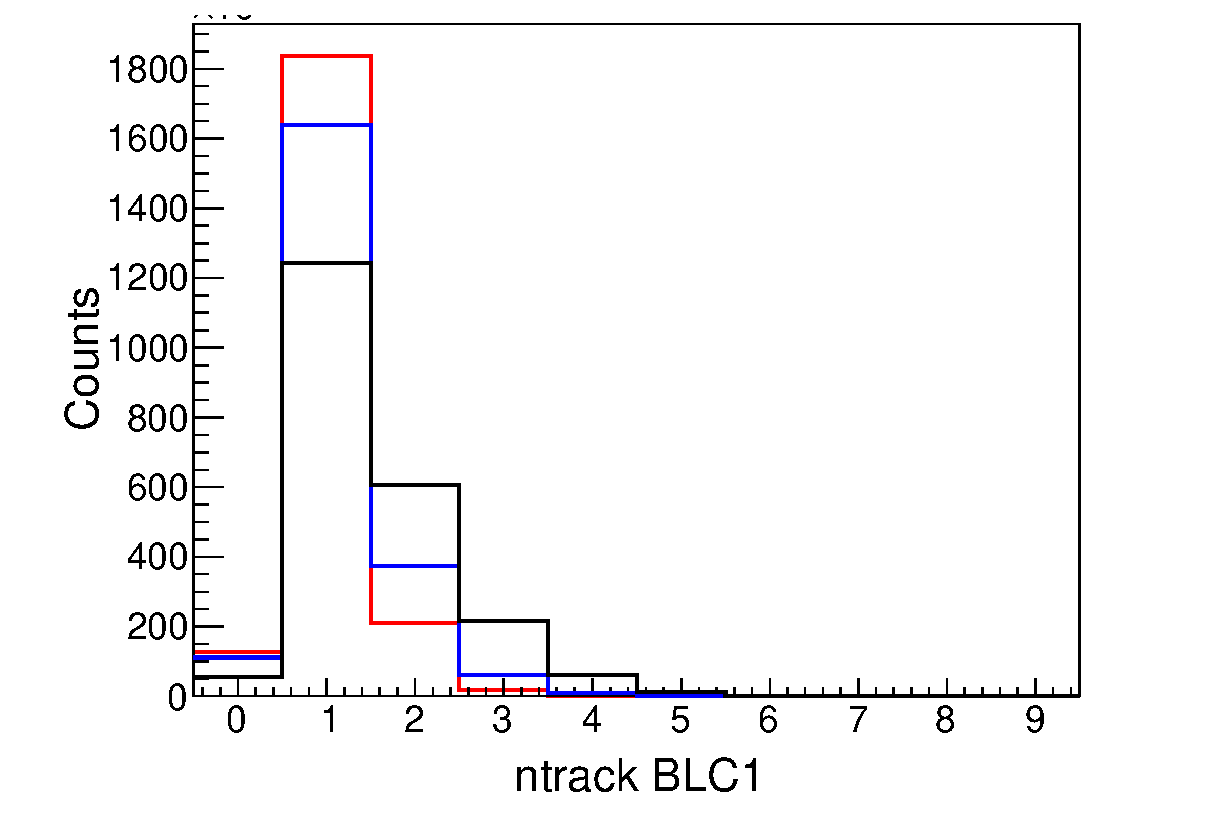
\includegraphics[width=2.5cm]{../pic/Run78/BL/nBLC1.eps}
    \end{figure}
  }{
    \begin{figure}
      \includegraphics[width=2.5cm]{../pic/Run78/BL/BLC1_time.eps}
    \end{figure}
  }{
    \begin{figure}
      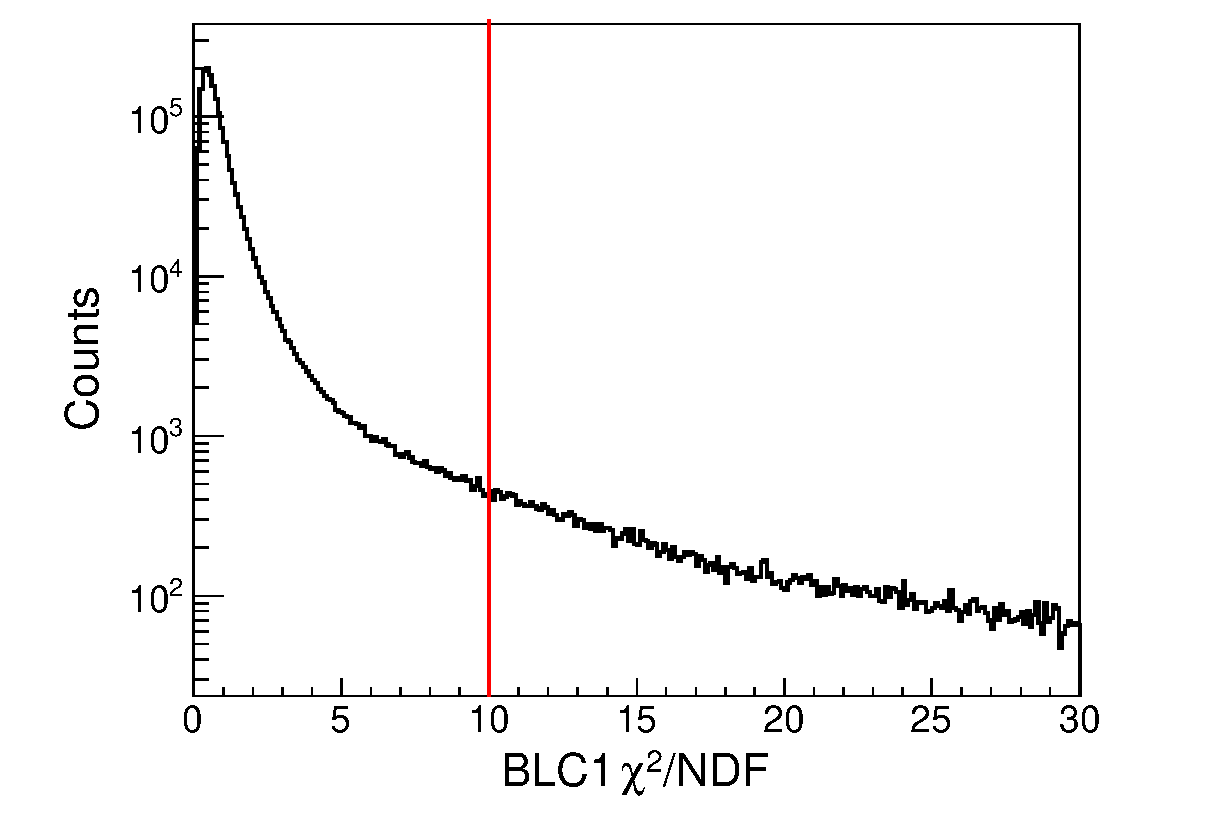
\includegraphics[width=2.5cm]{../pic/Run78/BL/BLC1_chi2.eps}
    \end{figure}
  }
  \centering
  \tiny
  BPC単体の解析とビーム選別はp.\pageref{page:BLC}のBLCと同様

  \begin{tabular}{cc}
    \begin{minipage}{0.5\hsize}
      \begin{figure}
        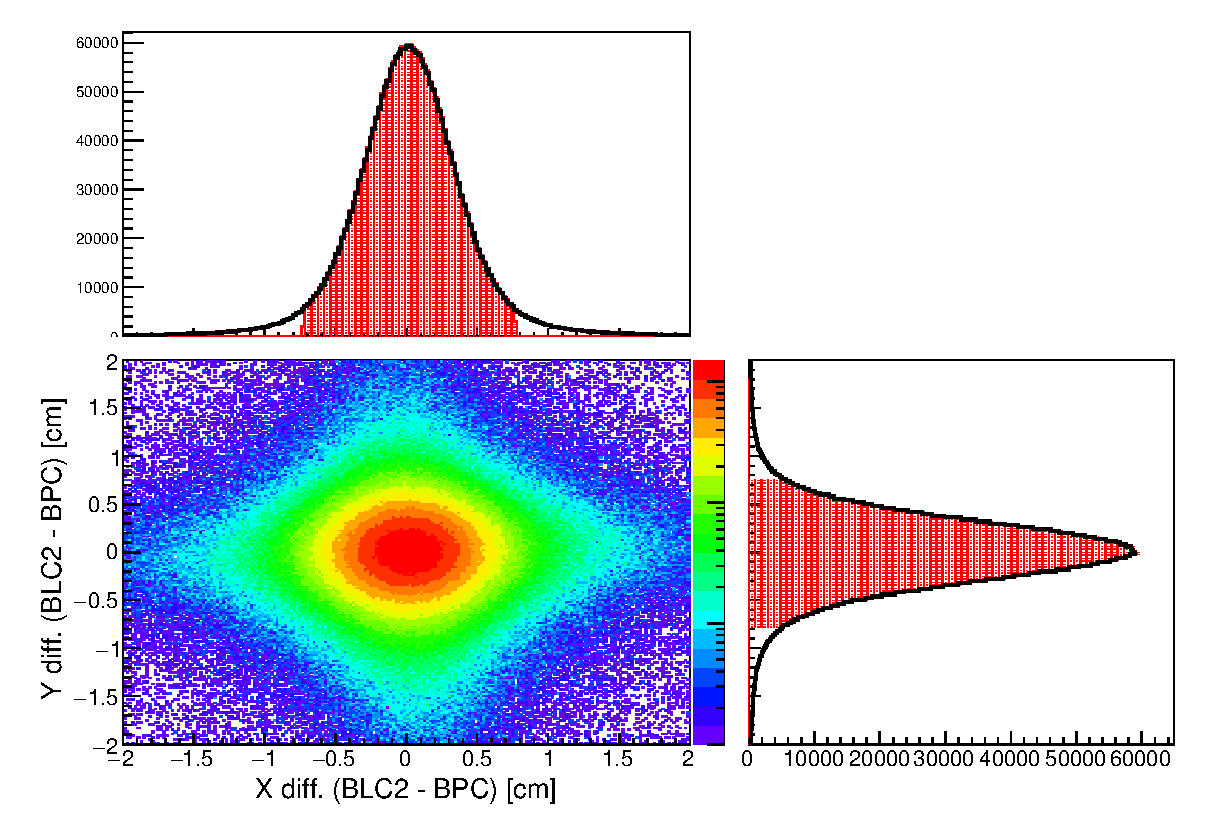
\includegraphics[width=4cm]{../pic/Run78/BL/BLC2BPC.eps}
      \end{figure}
      \vspace{-5mm}
      \centering
      BLC2とBPCの位置の違い、\\BLC2とBPCの中心点に外装して評価してある
    \end{minipage}

    \begin{minipage}{0.5\hsize}
      \begin{figure}
        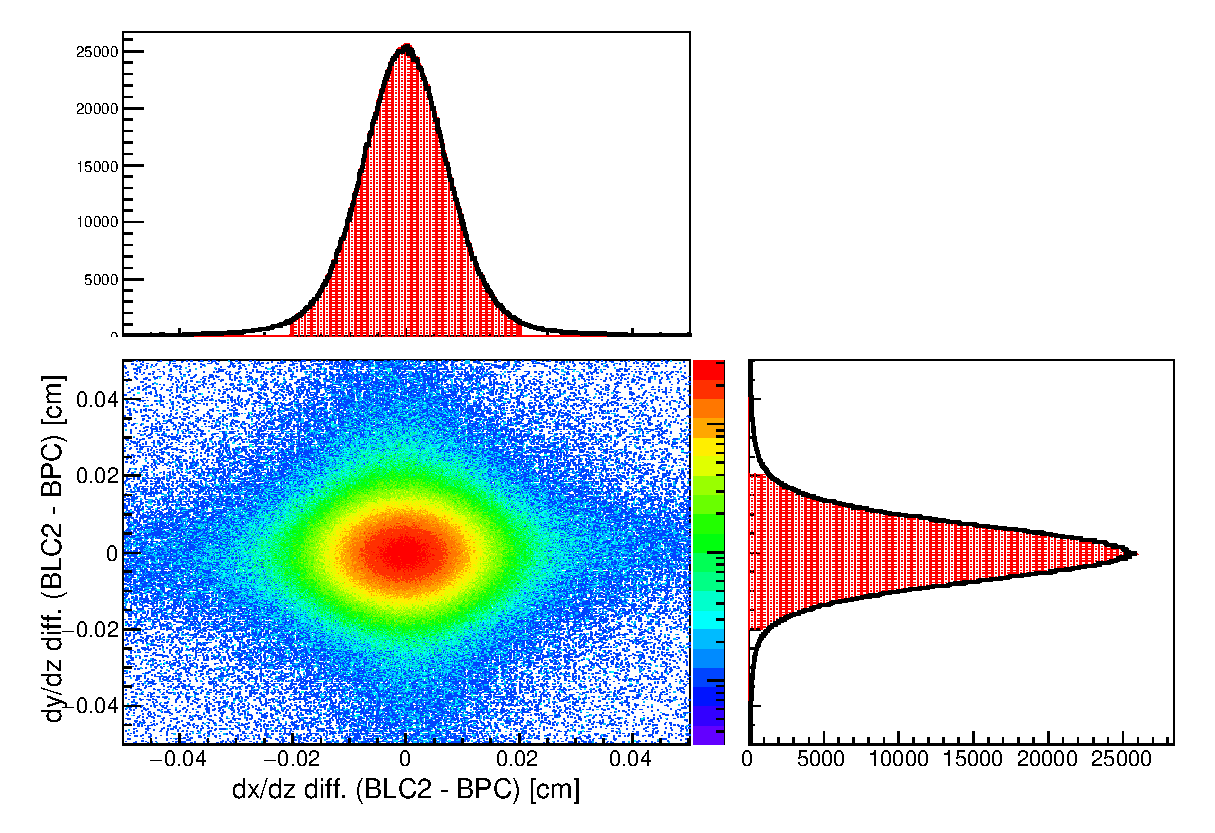
\includegraphics[width=4cm]{../pic/Run78/BL/BLC2BPC_dir.eps}
      \end{figure}
      \vspace{-5mm}
      \centering
      BLC2とBPCのトラックの向きの違い
    \end{minipage}
  \end{tabular}
  \centering
  \scriptsize
  \vspace{3mm}\\
  BLC2とBPCの接続は位置、向きとも$3\sigma$の範囲内(赤領域)で接続できることを要求する。
\end{frame}
